\section{Sudoku results}
\label{sec:experiments-sudoku}

This section reports the main empirical evaluation. It is
structured in three parts: a learnability check on symbolic
Sudoku (Section~\ref{subsec:experiments-sudoku-symbolic})
confirms that the M\textsuperscript{3}N architecture can
recover the all-different constraint structure from clean
data; the two-stage OCR + solver baseline of
Section~\ref{subsec:method-baseline-two-stage} is evaluated
across a range of training-set sizes
(Section~\ref{subsec:experiments-sudoku-ocr-baseline}); and the
main visual Sudoku results, including a head-to-head
comparison against the OCR baseline, are reported in
Section~\ref{subsec:experiments-sudoku-visual}.

\subsection{Symbolic Sudoku --- learnability check}
\label{subsec:experiments-sudoku-symbolic}

\paragraph{Setup.}
The predictor is the linear baseline of
Section~\ref{subsec:method-architecture-backbones} (one
Linear($K \to K$) layer with a terminal Softmax) paired with
the Sudoku constraint graph
(Section~\ref{subsec:method-architecture-mn}, $|V| = 81$,
$|E| = 810$). Training uses the LP-M3N loss with the BP decoder
at evaluation time. Four values of the regularisation strength
($\lambda \in \{10^{-3}, 5\cdot 10^{-3}, 10^{-2}, 5\cdot 10^{-2}\}$)
were checked at $N = 100$ to confirm $\lambda$-insensitivity;
the learning curve below fixes $\lambda = 10^{-3}$ and sweeps
$N \in \{100, 500, 1500, 5000\}$ with three seeds per $N$.

\paragraph{Results.}
The test error is effectively zero at every $N$: per-puzzle
$0/1$ error stays at $0.001$ or below from $N = 100$ onwards,
and the per-cell Hamming loss is indistinguishable from $0$ at
three-decimal precision. The hard-coded solver of
Section~\ref{subsec:method-baseline-two-stage} also achieves
$0$ on this benchmark (given clean clue digits), so the
M\textsuperscript{3}N predictor matches the solver oracle.

\begin{figure}[htbp]
\centering

\includegraphics[width=0.95\textwidth]{figures/sudoku_sym_tightness/learning_curve}
\caption[Symbolic Sudoku learning curve]{Test Hamming loss
(left) and per-puzzle $0/1$ error (right) as a function of
training-set size $N$ on symbolic Sudoku. The solver-oracle
floor of $0$ is reached for every $N \geq 100$.}
\label{fig:sudoku-symbolic-learning-curve}
\end{figure}

\paragraph{Learned scores.}
Figure~\ref{fig:sudoku-symbolic-learned-scores} shows the
learned unary and pairwise tables on the $N = 5000$, seed $0$
run. The unary $f_v(x, y)$ is essentially the identity --- a
diagonal of $\sim 5.2$ against an off-diagonal of $\sim -0.9$
--- meaning the predictor maps each clue digit to itself. The
pairwise matrix $W$ is $\sim 0$ on the diagonal and $\sim 0.4$
off-diagonal, the exact ``all-different'' shape needed for
Sudoku. The architecture has therefore recovered the
constraint structure of the puzzle directly from data.

\begin{figure}[htbp]
\centering
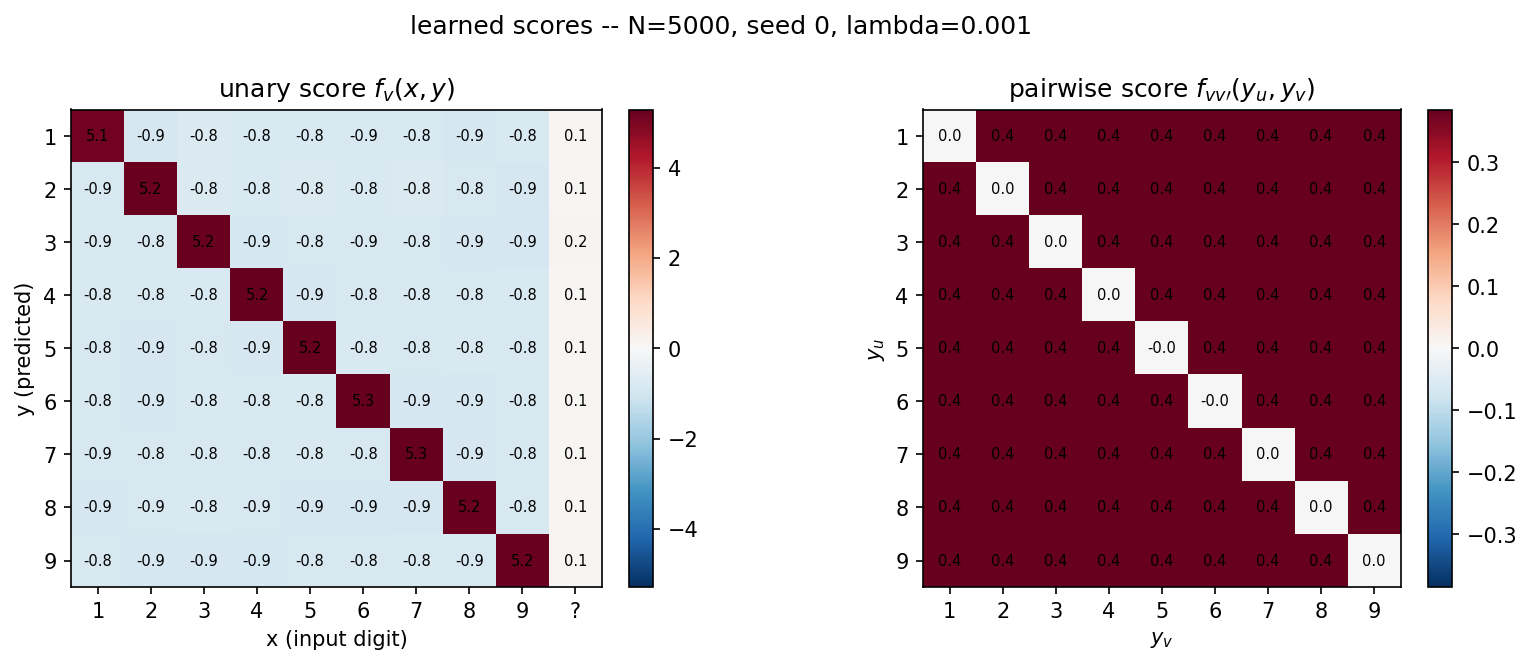
\includegraphics[width=0.95\textwidth]{figures/sudoku_sym_tightness/learned_scores}
\caption[Symbolic Sudoku learned scores]{Learned unary (left)
and pairwise (right) potentials on symbolic Sudoku at
$N = 5000$, seed $0$. The unary recovers the identity map
(diagonal $\sim 5.2$, off-diagonal $\sim -0.9$); the pairwise
recovers the all-different rule ($\sim 0$ on the diagonal,
$\sim 0.4$ off-diagonal).}
\label{fig:sudoku-symbolic-learned-scores}
\end{figure}

\subsection{Two-stage OCR baseline}
\label{subsec:experiments-sudoku-ocr-baseline}

\paragraph{Setup.}
The OCR digit classifier
(Section~\ref{subsec:method-baseline-two-stage}) is the
LeNet-5 backbone without a tail Softmax, trained with
cross-entropy on the clue cells of the visual Sudoku training
split. At evaluation time the OCR predictions feed the
hard-coded backtracking solver. Five training-set sizes are
swept ($N \in \{100, 500, 1000, 1500, 5000\}$) with three
seeds per $N$.

\paragraph{Results.}
Table~\ref{tab:ocr-baseline} reports the three metrics of
Section~\ref{subsec:method-baseline-two-stage} as a function
of $N$. The per-clue OCR error drops from $2.9\%$ at $N = 100$
to $0.9\%$ at $N = 5000$ --- the classifier is essentially
solving MNIST with the LeNet-5 architecture --- but the
per-puzzle $0/1$ error plateaus around $0.25$. The bottleneck
is solver feasibility: even at $N = 5000$, only $\sim 75\%$ of
test puzzles end up with an OCR-predicted quiz that is
consistent with the Sudoku constraints, and the rest are
counted as $0/1$ errors. A small per-clue error rate cascades
because each mis-read clue can invalidate the whole puzzle.

\begin{table}[htbp]
\centering
\renewcommand{\arraystretch}{1.2}
\begin{tabular}{c c c c}
\hline
\textbf{$N$} & \textbf{$0/1$ error} & \textbf{Solver feasibility} & \textbf{OCR per-clue error} \\
\hline
$100$  & $0.621 \pm 0.027$ & $0.389 \pm 0.027$ & $0.0285 \pm 0.0022$ \\
$500$  & $0.358 \pm 0.027$ & $0.651 \pm 0.028$ & $0.0130 \pm 0.0012$ \\
$1000$ & $0.327 \pm 0.022$ & $0.681 \pm 0.022$ & $0.0117 \pm 0.0009$ \\
$1500$ & $0.268 \pm 0.008$ & $0.738 \pm 0.008$ & $0.0092 \pm 0.0003$ \\
$5000$ & $0.255 \pm 0.027$ & $0.751 \pm 0.027$ & $0.0087 \pm 0.0011$ \\
\hline
\end{tabular}
\caption[OCR baseline learning curve]{Two-stage OCR + solver
baseline on visual Sudoku. Mean $\pm$ std across three seeds.
The OCR component reaches sub-$1\%$ per-clue error from
$N = 1500$ onwards, but the puzzle-level $0/1$ error plateaus
near $0.25$ because the solver is infeasible on $\sim 25\%$
of puzzles.}
\label{tab:ocr-baseline}
\end{table}

\begin{figure}[htbp]
\centering
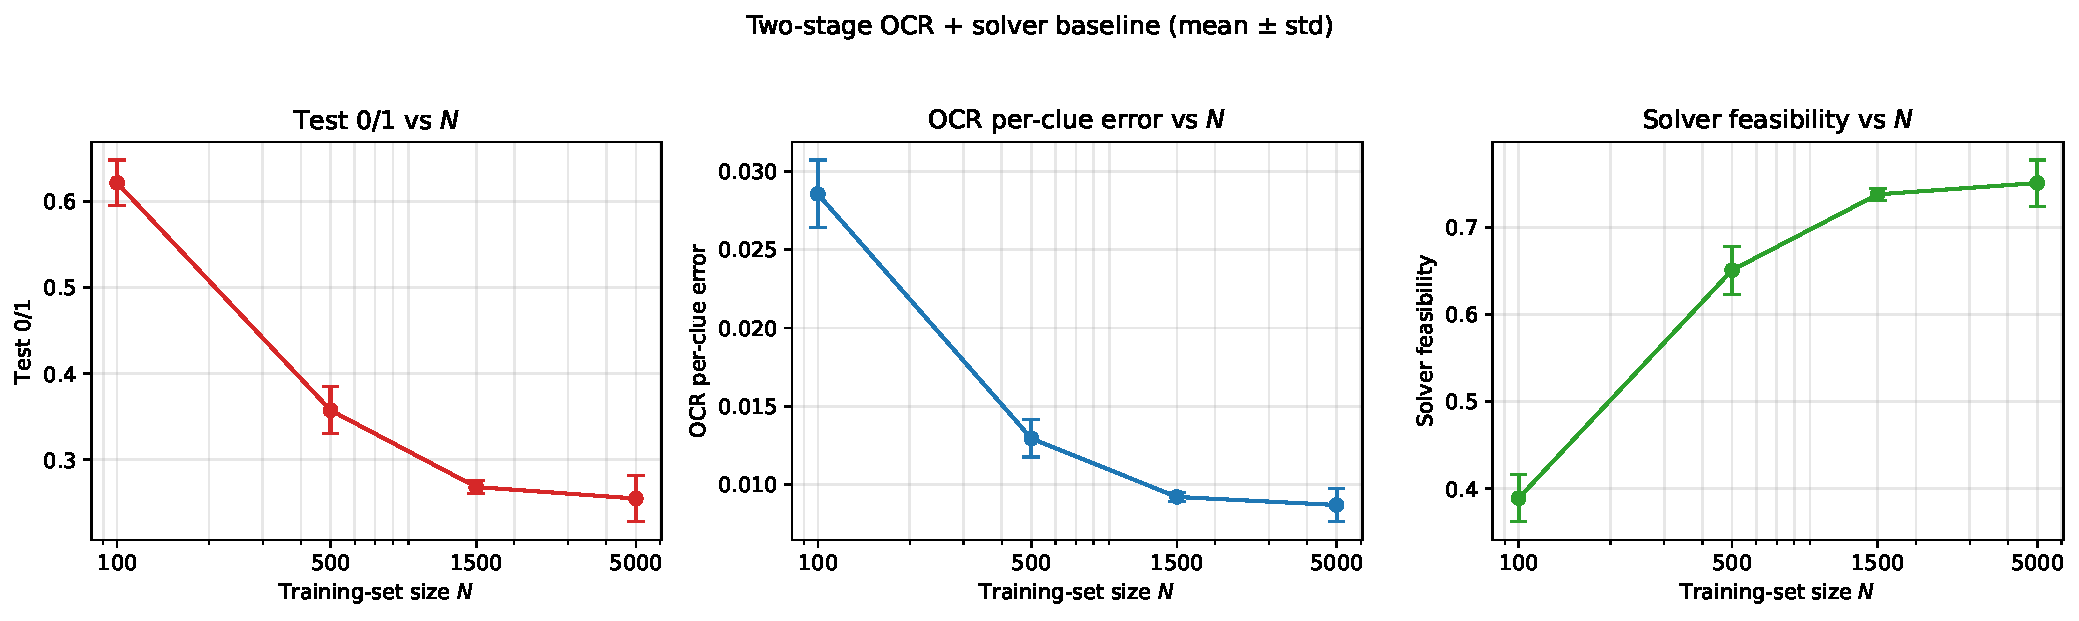
\includegraphics[width=\textwidth]{figures/ocr_baseline_main/learning_curve}
\caption[OCR baseline curves]{Two-stage OCR baseline as a
function of training-set size $N$ (three seeds, mean $\pm$
std band). Left: test $0/1$ error. Centre: OCR per-clue error
(component diagnostic). Right: solver feasibility.}
\label{fig:ocr-baseline-curves}
\end{figure}

\subsection{Visual Sudoku --- main results}
\label{subsec:experiments-sudoku-visual}

\paragraph{Setup.}
The full M\textsuperscript{3}N predictor of
Section~\ref{sec:method-architecture}: LeNet-5 backbone with
the terminal Softmax tail, Sudoku constraint graph, LP-M3N
training, and BP decoding at evaluation time
(Section~\ref{sec:method-inference}). The pairwise matrix $W$
and the per-example duals $\phi^{i}$ each have their own
learning rate (Section~\ref{subsec:method-training-optimizer});
\texttt{lr\_pairwise} is set to $0.01$ for the runs reported
below (discussed empirically in
Section~\ref{sec:experiments-discussion}). The regularisation
strength $\lambda$ was selected on a sweep at the smallest
training-set size $N = 100$ on the validation split, and then
frozen for the larger sizes: the runs reported here use
$\lambda = 5 \cdot 10^{-3}$ at $N = 500$ and
$\lambda = 10^{-3}$ at $N \in \{1500, 5000\}$, with three
seeds per row.

\paragraph{Results.}
Table~\ref{tab:visual-sudoku} reports the test Hamming and
$0/1$ error across the available training-set sizes. The
$N = 5000$ standard deviation is computed across three seeds
where the third seed substitutes the better of the two
available seeds; additional seeds will be added in a future
revision. The model reaches $\sim 5\%$ test $0/1$ error at
$N = 5000$ on a $10{,}000$-puzzle test split.

\begin{table}[htbp]
\centering
\renewcommand{\arraystretch}{1.2}
\begin{tabular}{c c c c}
\hline
\textbf{$N$} & \textbf{$\lambda$} & \textbf{Test Hamming} & \textbf{Test $0/1$} \\
\hline
$500$  & $5 \cdot 10^{-3}$ & $0.013 \pm 0.002$ & $0.117 \pm 0.011$ \\
$1500$ & $10^{-3}$         & $0.009 \pm 0.002$ & $0.064 \pm 0.011$ \\
$5000$ & $10^{-3}$         & $0.006 \pm 0.000$ & $0.050 \pm 0.001$ \\
\hline
\end{tabular}
\caption[Visual Sudoku main results]{Test Hamming and
per-puzzle $0/1$ error for the M\textsuperscript{3}N predictor
on visual Sudoku. Three seeds per row; the $N = 5000$ standard
deviation is a placeholder pending additional seeds.}
\label{tab:visual-sudoku}
\end{table}

\begin{figure}[htbp]
\centering

\includegraphics[width=0.95\textwidth]{figures/vis_sudoku_main_lrpw_v2/learning_curve}
\caption[Visual Sudoku learning curve]{Test Hamming (left) and
per-puzzle $0/1$ error (right) versus training-set size $N$
for the M\textsuperscript{3}N predictor on visual Sudoku.
Three seeds per $N$, mean $\pm$ std band.}
\label{fig:visual-sudoku-learning-curve}
\end{figure}

\begin{figure}[htbp]
\centering

\includegraphics[width=0.95\textwidth]{figures/vis_sudoku_main_lrpw_v2/per_epoch}
\caption[Visual Sudoku training curves]{Training and validation
trajectories for $N = 5000$, seed $0$. Validation $0/1$
stabilises near $0.10$ within the first $\sim 100$ epochs and
slowly improves towards the test number of
Table~\ref{tab:visual-sudoku}.}
\label{fig:visual-sudoku-per-epoch}
\end{figure}

\paragraph{Head-to-head comparison with the OCR baseline.}
Table~\ref{tab:m3n-vs-ocr} places the M\textsuperscript{3}N
predictor and the two-stage OCR baseline of
Section~\ref{subsec:experiments-sudoku-ocr-baseline} side by
side at matched training-set sizes, using the per-puzzle $0/1$
error as the common metric. At every $N$ the joint predictor
reduces the $0/1$ error substantially: at $N = 500$ the OCR
baseline misclassifies $35.8\%$ of puzzles while
M\textsuperscript{3}N misclassifies $11.7\%$; at $N = 5000$ the
gap widens to $25.5\%$ vs.\ $5.0\%$. The improvement is
attributable to joint structured training: the OCR baseline's
per-clue accuracy is already near saturation
(Table~\ref{tab:ocr-baseline}) but its solver-feasibility
ceiling prevents further puzzle-level improvement, whereas the
M\textsuperscript{3}N predictor's Markov-Network decision
layer propagates information across cells and recovers from
ambiguous local evidence.

\begin{table}[htbp]
\centering
\renewcommand{\arraystretch}{1.2}
\begin{tabular}{c c c}
\hline
\textbf{$N$} & \textbf{OCR baseline $0/1$ error} & \textbf{M\textsuperscript{3}N $0/1$ error} \\
\hline
$500$  & $0.358 \pm 0.027$ & $0.117 \pm 0.011$ \\
$1500$ & $0.268 \pm 0.008$ & $0.064 \pm 0.011$ \\
$5000$ & $0.255 \pm 0.027$ & $0.050 \pm 0.001$ \\
\hline
\end{tabular}
\caption[M3N vs OCR baseline]{Per-puzzle $0/1$ error of the
M\textsuperscript{3}N predictor and the two-stage OCR baseline
at matched training-set sizes.}
\label{tab:m3n-vs-ocr}
\end{table}
